\chapter{Calcul des matrices source-récepteur par un modèle lagrangien adjoint}

\todoin{
	\textbf{TODO CHAPITRE 4}
	\begin{itemize}
		\item Reprendre suite eq.(4) du papier AE pour introduire l'alternative backward
	\end{itemize}
}
L'étude de cas sur l'expérience FFT07 présentée dans le Chapitre 3 a montré que la charge de calcul de la procédure d'estimation du terme source est en grande majorité focalisée sur le calcul de la matrice source-récepteur. Cette étape nécessite une quantité d'appels au modèle de dispersion égale au nombre de particules échantillonnées par itération multiplié par le nombre d'itérations, soit en pratique 1000 instances dans le cas de FFT07. \\

Si pour les cas les plus simples il est possible de se limiter à des modèles de dispersion suffisamment rapides, la situation change dès qu'il s'agit de considérer un contexte plus élaboré, avec des outils de calculs permettant certes une meilleure représentation des phénomènes de dispersion, mais dont l'exécution devient bien plus coûteuse en termes d'implémentation et de temps de calcul. \\

L'objet de ce chapitre est ainsi de présenter une façon d'optimiser le calcul des matrices source-récepteur lorsque celui-ci doit faire appel à un code de dispersion plus complexe que le modèle à bouffées gaussiennes précédemment évoqué. La présentation de cet outil de calcul constituera la première partie de ce chapitre, avec notamment une explication de son fonctionnement, puis une présentation de son intégration optimale à la chaîne de calcul et d'estimation existante. La suite du chapitre se concentrera sur les aspects pratiques autour de la mise en application de cette méthodologie améliorée, avec la présentation des résultats sur plusieurs cas-tests de simulation.


\section{Le code de calcul PMSS}

\subsection{L'approche lagrangienne de la dispersion atmosphérique}
\label{part_lagrangian}

Pour les modèles dits eulériens, la résolution du problème de la dispersion d'un polluant dans l'atmosphère passe par la construction d'un maillage sur le domaine étudié, afin de pouvoir observer l'évolution des concentrations du polluant porté par les mouvements de l'air. 

Le point de vue lagrangien est différent: il s'agit ici de résoudre un système d'équations dans un repère lié au déplacement de la masse d'air contenant le polluant. Pour cela, on représente le panache sous la forme d'un ensemble de \textit{particules lagrangiennes}\footnote{Afin d'éviter toute confusion avec les particules statistiques dont il est fait référence dans le cadre de l'algorithme AMIS, nous utiliserons la dénomination  de \textit{particule lagrangienne} abréviée par PL dans la suite du texte. Nous conservons le terme de \textit{particule} pour désigner les échantillons issus de l'AMIS.}, chacune étant porteuse d'une masse élémentaire du polluant considéré. Le principe d'un modèle lagrangien consiste ainsi à étudier les trajectoires de ces éléments discrets dans le domaine au fil du temps.

Le fait de modéliser le panache par un ensemble de PL permet de tenir compte de la nature stochastique de leur déplacement, qui traduit la variabilité inhérente aux processus de turbulences auxquels est soumis le panache: on parle d'ailleurs plus précisément de \textit{modèle lagrangien stochastique}. On va ainsi travailler sur une équation de transport portant sur la densité de probabilité associée à chaque trajectoire. Plus formellement, d'après \cite{Flesch1995}, la formulation classique régissant un modèle de dispersion lagrangien se présente sous la forme d'une équation de Langevin, qui s'écrit: 

\begin{equation}
	\begin{split}
		du_i &= a_i(\Vecx, \Vecu, t)dt + b_{i,j}(\Vecx, \Vecu, t)d\xi_j  \\
		dx_i &= u_i dt
	\end{split}
	\label{eq_langevin}
\end{equation}
où:
 \begin{itemize}
	\item $\Vecx = (x, y, z)$ est la position de la PL  définie par un repère spécifique: $x$ suit l'axe du vent, $y$ suit l'axe perpendiculaire au vent, et $z$ désigne l'élévation verticale classique. 
	\item $\Vecu$ est la vitesse d'écoulement à laquelle est soumise la PL: $\Vecu = (u, v, w)$ où les composantes respectives de ce vecteur suivent les mêmes axes que $\Vecx$.
	\item $a_i$ et $b_{i,j}$ sont des fonctions spécifiques de $(\Vecx, \Vecu, t)$.
	\item $d\xi_j$ est un incrément aléatoire suivant une distribution gaussienne de moyenne nulle et de variance $dt$.\\
\end{itemize}

L'expression des fonctions $a_i$ et $b_{i,j}$ varie selon les hypothèses que l'on se fixe sur la nature de la turbulence: une présentation plus détaillée de leur calcul est disponible dans \cite{Wilson1996}. Une fois que ceux-ci sont définis,l'équation \eqref{eq_langevin} est discrétisée et sa résolution permet de calculer un ensemble de trajectoires de PL émanant d'une source dont les paramètres sont connus. Les concentrations volumiques moyennes simulées sont alors obtenues par la somme des particules présentes dans un volume élémentaire $d\Vecx$ autour du point d'observation $\Vecx$ durant un certain temps de résidence. En d'autres termes, on peut écrire la concentration moyenne au point $\Vecx$ et à l'instant $t$ comme étant : 

\begin{equation}
	C(\Vecx, t) = \int _{-\infty}^{t} \int_{V} S(\Vecx',t')p(\Vecx, t | \Vecx', t')d\Vecx'dt
	\label{eq_c_moyen_lagrangien}
\end{equation}
où $V$ est le volume défini par le domaine d'étude, $S(\Vecx',t')$ est la distribution de la source, et $p(\Vecx, t | \Vecx', t')$ est la densité de probabilité sur la position $\Vecx$ et l'instant $t$ des PL de position initiale $\Vecx'$ à l'instant $t'$. \\

\begin{figure}
	\centering
	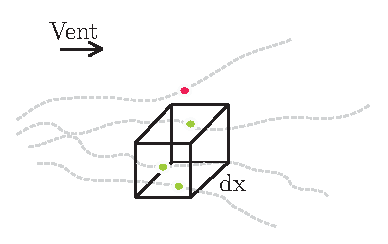
\includegraphics[width=0.65\textwidth]{lagrangian_ok}
	\caption{Principe du modèle lagrangien: la concentration en $\Vecx$ s'obtient par la somme des PL (en vert) traversant le volume élémentaire $d\Vecx$ durant un certain temps de résidence.}
	\label{fig_schema_lagrangien}
\end{figure}

Afin de calculer le champ d'écoulement auquel sont soumises les PL, plusieurs méthodes sont disponibles. Il est par exemple possible de résoudre les équations de la mécanique des fluides via un outil de simulation de type CFD, ce qui permet une modélisation fine des phénomènes physiques mis en jeu. Une autre possibilité consiste à avoir recours à une simulation dite \textit{CFD simplifiée}, où le champ de vent est interpolé à partir des mesures d'une ou plusieurs stations météorologiques tout en prenant en compte la topographie du terrain. C'est cette dernière approche qui est employée dans les outils de calcul du CEA et d'ARIA Technologies, et que nous présentons dans le chapitre suivant. \\

\subsection{La chaîne de calcul SWIFT-SPRAY}

L'outil \textit{Parallel Micro-SWIFT-SPRAY} (PMSS) est une chaîne de calcul constituée de deux éléments distincts: un outil de CFD simplifiée (SWIFT) et un modèle de dispersion lagrangien stochastique (SPRAY). Il est généralement appliqué dans des études à petite échelle (par exemple, au niveau d'un quartier), mais grâce à sa version parallèle, il a récemment été utilisé sur des domaines plus grands, à l'exemple du cas AirCity (REF) où le modèle a été exécuté sur l'ensemble de la ville de Paris.\\

\subsubsection{SWIFT}

Le modèle SWIFT permet de produire des champs de vent 3D en exploitant différents types de données météorologiques sur un même site (profils de vent et de température, stations de mesures, sorties de modèles météorologiques de prévision). Il permet notamment de prendre en compte la topographie du milieu, la présence d'obstacles tels que des bâtiments, l'occupation des sols ou encore l'influence de la stabilité atmosphérique. Son fonctionnement peut être résumé en quatre étapes :  \\

\begin{enumerate}
	\item Dans un premier temps, les mesures météorologiques reçues en entrée sont interpolées sur les différents points constituant une version discrétisée du domaine.
	\item Dans un deuxième temps, l'effet des obstacles présents dans le domaine sur l'écoulement sont modélisés via la création de zones spécifiques dans le voisinage de ces obstacles où le champ de vitesse est calculé de façon spécifique.
	\item La troisième étape consiste à ajuster le champ de vent en appliquant un principe de conservation de la masse.
	\item Enfin, la dernière étape consiste à calculer la turbulence intrinsèque à l'écoulement modélisé.\\
\end{enumerate}

En sortie de cet enchaînement de calculs, on obtient un champ de vent 3D qui peut alors directement être exploité par le modèle de dispersion SPRAY.

\begin{figure}
	\centering
	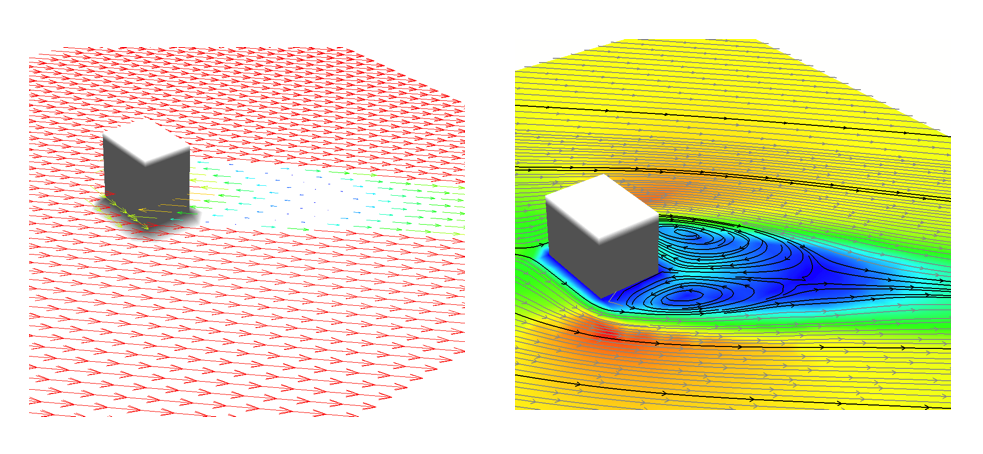
\includegraphics[width=0.75\textwidth]{swift_exemple}
	\caption{Exemple de calcul d'un champ de vent autour d'un obstacle avec SWIFT, avant (à gauche) et après (à droite) l'ajustement du champ}
	\label{fig_swift_exemple}
\end{figure}

\subsubsection{SPRAY}

SPRAY est un modèle de dispersion lagrangien stochastique dont les principes de base suivent les mécanismes présentés à la section \ref{part_lagrangian}. Plusieurs fonctionnalités supplémentaires sont implémentées dans SPRAY, telles que: \\

\begin{itemize}
	\item le "rebond" des particules sur les obstacles,
	\item le calcul de doses pour les sources radioactives,
	\item la prise en compte des différents types de dépôts (secs ou humides).\\
\end{itemize}

\begin{figure}[h!]
	\centering
	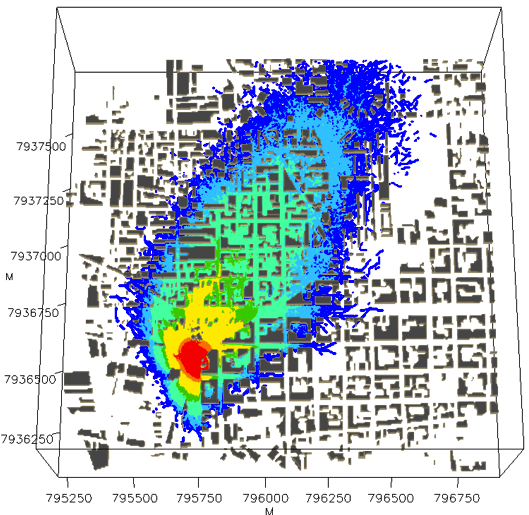
\includegraphics[width=0.65\textwidth]{spray_exemple}
	\caption{Exemple de champ de concentration calculé par SPRAY dans un domaine de type urbain}
	\label{fig_spray_exemple}
\end{figure}

La combinaison de SWIFT et SPRAY permet ainsi de calculer un champ de concentration sur le domaine étudié, connaissant les paramètres du terme source qui sont soumis en entrée du modèle SPRAY. Dans ce chapitre, la chaîne de calcul PMSS est utilisée à a fois pour : \\

\begin{itemize}
	\item simuler un rejet induit par une source que l'on va chercher à retrouver: pour cela, on va récupérer les valeurs de concentration sur un nombre fini de points du domaine que nous définirons comme étant les valeurs d'observation fournies par les capteurs,
	\item à construire les matrices source-récepteur nécessaires au processus d'estimation du terme source.\\
\end{itemize}

Sur ce dernier point, comme il s'agit désormais de travailler avec un outil de simulation relativement complet, et nécessitant \textit{de facto} des temps de calculs plus importants, il devient nécessaire d'optimiser le schéma algorithmique de l'estimation des paramètres de la source. Nous détaillons l'approche choisie dans la partie suivante.


\subsection{Dualité \textit{forward-backward}}

\subsection{Intégration de RetroSPRAY au processus d'estimation}

\section{Exemple d'application en rase campagne}

\subsection{Présentation du cas-test}

\subsection{Analyse paramétrique sur $\varObs$}

\subsection{Analyse paramétrique sur $\varQ$}

\subsection{Modularité du réseau de capteurs}

\section{Exemple d'application à un cas urbain}

\subsection{Présentation du cas-test}

\subsection{Procédure de \textit{fitting} de la loi de proposition}

\subsection{Résultats}





